\phantomsection


% Is it possible to keep my translation together with original text?
% https://tex.stackexchange.com/questions/5076/is-it-possible-to-keep-my-translation-together-with-original-text
\chapter[\lang{Basic concepts and Related works}{Conceitos básicos e Trabalhos relacionados}]
{
    \lang
    {Basic concepts and Related works}
    {Conceitos básicos e Trabalhos relacionados}
}
\label{sec:related}

\begin{flushright}
    \englishword{ }
\end{flushright}


% Multiple-language document - babel - selectlanguage vs begin/end{otherlanguage}
% https://tex.stackexchange.com/questions/36526/multiple-language-document-babel-selectlanguage-vs-begin-endotherlanguage
In this chapter we present the basic concepts for this thesis in Section \ref{sec:basic_concepts}. In Section \ref{sec:related_measures} we present a review on trajectory similarity measures, where the section \ref{sec:related_raw} presents measures for raw trajectory similarity and the section \ref{sec:related_semantic} presents measures for semantic trajectory similarity.

\section{Basic concepts} \label{sec:basic_concepts}
In this section we present basic concepts related to trajectories in Section \ref{sec:trajectories} and basic concepts about similarity measures and some evaluation techniques in Section \ref{sec:similarity_measures}.

\subsection{Trajectories}\label{sec:trajectories}
There are two important concepts that need to be explained and defined: raw trajectory and semantic trajectory.
A raw trajectory is a discrete representation of the movement of an object that can be defined as a time-ordered finite sequence of space-time points, as formalized in Definition \ref{def:raw_trajectory}. 

\begin{definition}[Raw Trajectory] \label{def:raw_trajectory}
A raw trajectory is a time-ordered sequence of points in the form T = $<p_1,...,p_n>$ where point p\textsubscript{k} $\in$ T is a tuple p\textsubscript{k} = ($x,y,t$), where $x,y$ represent the spatial location of the moving object at a time instant $t$.
\end{definition}

Figure \ref{fig:example_raw_trajectory} illustrates an example of a raw trajectory. The spatial coordinates are annotated next to the trajectory points and the time instants can be seen as the index associated to each point. For instance, the first point of the trajectory in the figure is located at the coordinates $(2,3)$ at time instant $1$.

In 2007 Alvares \cite{alvares2007model} and Spaccapietra \cite{Spaccapietra:2008:CVT:1347466.1347785} proposed a new representation for trajectories, called semantic trajectory. A semantic trajectory is a time-ordered sequence of \emph{stops} and \emph{moves}, where the \emph{stops} are the most relevant parts of the trajectory.
In this work we formally define semantic trajectory considering its sequence of stops and moves, which is an enriched extension of the definition presented in \cite{Spaccapietra:2008:CVT:1347466.1347785}:

\begin{definition}[Semantic Trajectory]
\label{def:semantic_trajectory}
A semantic trajectory  \break
$S=\langle s_1, m_1, s_2, m_2, s_3,m_3, ...., s_k, m_k, s_{k+1} \rangle$ is a time ordered sequence of stops and moves, where each stop $s_i$ has a set of attributes $\{d_{s1}, d_{s2}, ...,d_{sq}\}$ characterizing it according to q-dimensions, and each move $m_j$  has a set of attributes $\{d_{m1}, d_{m2}, ...,d_{mr}\}$ characterizing it according to r-dimensions. 
\end{definition}

Figure \ref{fig:related_semantic_trajes} shows a semantic trajectory $S$ representing the movement of a professor. In this example the semantic trajectory is enriched with the name of the place where the \emph{stop} occurred, the category of the place, its spatial coordinates, and the time interval that the \emph{stop} happened. The \emph{move} is enriched with the name of the street where the object moves, the traveled distance, and the average speed during the \emph{move}.

\begin{figure}[h]
\centering
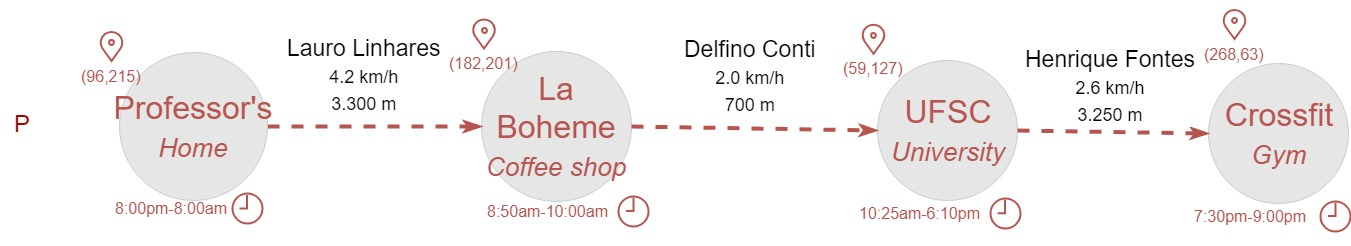
\includegraphics[width=0.85\textwidth]{Related_Works/Single_Semantic_trajectorie.jpg}
\caption{\label{fig:related_semantic_trajes}A semantic trajectory $S$ representing the movement of a professor}
\end{figure}

\subsection{Similarity measures and evaluation techniques}\label{sec:similarity_measures}
To compare two trajectories we use a similarity measure. In this thesis we use the intuitive concept of similarity stated in \cite{lin1998information}, where two objects $A$ and $B$ are more similar as the commonality between each other increases, and they are less similar as their differences increase. We formalize the similarity measure concept according Definition \ref{def:similarity_measure} introduced by \cite{lin1998information}:

\begin{definition}[Similarity Measure]
\label{def:similarity_measure}
A similarity measure on two objects $A$ and $B$ is a function $sim: A \times B \to [0,1]$, such that the objects are more similar when the score returned by $sim(A, B)$ increases.
\end{definition}

{To evaluate how well a measure computes the similarity of two trajectories we use information retrieval evaluation techniques. In this thesis we use the Precision-Recall approach, computing the Mean Average Precision (MAP) and the Area Under the Curve (AUC) values, as stated in }\cite{BaezaYatesRibeiroNeto2011}{. In the Precision-Recall approach, the measure is evaluated as how precise is the information retrieval in each recall level, where each recall level is the recover of the relevant trajectories in the whole dataset. The Mean Average Precision (MAP) value of a Precision-Recall measure is the average precision in all recall levels. The Area Under the Curve (AUC) value is calculated by constructing the Precision-Recall curve and calculating the area under this curve.}

\section{Related Trajectory Similarity Measures} \label{sec:related_measures}

Similarity measures have been proposed for several data processing and analysis techniques, such as outlier detection, top-K similarity queries, clustering, and others. In the context of trajectories, several similarity measures were proposed for both raw trajectories and semantic trajectories. In this section, we present a literature review on similarity measures of raw trajectories in Section \ref{sec:related_raw} and Section \ref{sec:related_semantic} presents the similarity measures for semantic trajectories.


\subsection{Related works on raw trajectory similarity measures} \label{sec:related_raw}
As presented in Section {\ref{sec:basic_concepts},} a raw trajectory is a time-ordered sequence of points containing a spatial coordinate and a timestamp. For this reason, existing measures developed for generic time-ordered sequences or time-series can be applied to raw trajectories, even though they were not originally developed for this. At the beginning of this section, we present a distance measure proposed for time-series  called Dynamic Time-Warping (DTW)\cite{berndt1994using} that was adapted to work with raw trajectory data in the work of \cite{ten2007multi}, creating the Multidimensional DTW (MD-DTW). Then we present similarity measures developed for raw trajectories which were adapted from more general similarity measures such as \textit{Discrete Fr{\'e}chet Distance} \cite{eiter1994computing}, \textit{w-constrained discrete Fr{\'e}chet Distance} (wDF) \cite{Ding:2008:ESJ:1440463.1440989}, \textit{Longest Common Subsequence} (LCSS) \cite{vlachos2002discovering}, \textit{Edit Distance on Real sequence} (EDR) \cite{Chen:2005:RFS:1066157.1066213} and after, the similarity measure proposed exclusively for raw trajectories called \textit{Uncertain Movement Similarity} (UMS) \cite{Furtado-UMS-2018}.

Throughout this section, we use a set of symbols to denote hypothetical trajectories. Table \ref{tab:symbols} summarizes the symbols used in this section.

\begin{table}[!h]
    \centering
    \resizebox{\linewidth}{!}{%
        \begin{tabular}{c|c}
             Symbol & Meaning  \\
             \hline
             $P$, $Q$ and $R$ & Trajectories \\
             $m$ and $n$ & Number of points of trajectories $P$ and $Q$, respectively \\
             $d_i$ & \emph{i}th-dimension of data in a point \\
             $window$ & Size of the window \\
             $k$ & Number of \emph{moves} in a semantic trajectory \\
             $\epsilon$ & Distance threshold between two points matching \\
             $x,y$ & Spatial coordinates \\
             $dist()$ & Distance function
        \end{tabular}
    }
    \caption{Symbol meanings}
    \label{tab:symbols}
\end{table}

An early proposed distance measure is the \emph{Dynamic Time Warping} (DTW) \cite{berndt1994using}, developed for time-series. DTW is used to find the best match between the points of two time-series independent of their sizes. It creates a matrix with all possible pairs of points of the time-series with the pairwise distances as the entries.
The distance between two trajectories is given by the sum of the entries of the minimum contiguous path in the matrix, where the minimum contiguous path is the best alignment between the sequences. Because DTW sums the distances between all points, it is sensitive to noise. For example, when a trajectory $P$ has a point that is significantly distant from all points of the trajectory $Q$, even if all the other points of $P$ and $Q$ are close, their distance will be dominated by the distant point. A recursive formalization of DTW is presented in Equation \ref{func:DTW}.

\begin{equation}
\label{func:DTW}
  DTW(P, Q) = 
    \begin{cases} 
        0 & \text{if } m = n = 0\\ 
      \infty & \text{if } m = 0 \text{ or } n = 0\\ 
      dist(p_1, q_1) + min( & otherwise\\
      DTW(<p_2...p_m>,<q_2...q_n>),\\
      DTW(<p_2...p_m>, Q), \\
      DTW(P, <q_2...q_n>)) &
    \end{cases}
\end{equation}

The \emph{Multidimensional DTW} (MD-DTW) \cite{ten2007multi} extends DTW for dealing with sequences whose points have more than one dimension. MD-DTW normalizes the distance in the different dimensions and then creates a matrix with entries as the sum of the distances in all dimensions. Finally, it runs DTW over the matrix and finds the minimum contiguous path, that is, the path in the matrix connecting all points of both trajectories with minimum distance. Figure \ref{fig:related_trajes_DTW} illustrates the computation of MD-DTW between trajectories $P$ and $Q$. Its distance is calculated as the sum of the minimum contiguous path between points of $P$ and $Q$, i.e. the sum of all dashed lines.

\begin{figure}[ht]
\centering
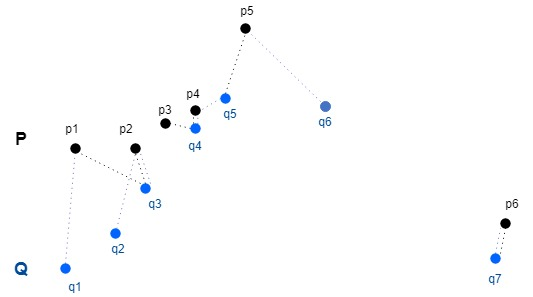
\includegraphics[width=0.45\textwidth]{Related_Works/related_trajes-DTW.jpg}
\caption{\label{fig:related_trajes_DTW}MD-DTW score is the sum of distances of the minimum contiguous path between $P$ and $Q$ trajectories (dashed lines)}
\end{figure}

In the work of \cite{Shokoohi-Yekta2017} is proposed an \emph{adaptive} DTW (DTWa) to multidimensional data. This adaptive approach is based on how the DTW computes the distance between two multidimensional sequences: (i) if the distance in each dimension is computed independently and summed at end; or (ii) if the distance between of each multidimensional point is computed taking into account all dimensions together. The \emph{adaptive} term comes from the decision of which approach is more reliable, by using a training dataset of multidimensional sequences and performing an evaluation.

\emph{Discrete Fr{\'e}chet Distance} was proposed in \cite{eiter1994computing} as an adaption of the classical Fr{\'e}chet Distance \cite{Frechet1906} to work with trajectories. This distance is also called the \emph{coupling} \emph{distance}, where the distance of two trajectories is the maximum distance of all aligned trajectory points on both trajectories. In this sense, an aligned trajectory point is a pair of points, where each point of one trajectory is \emph{coupled} with one and only one point of the other trajectory, taking into account the order of the points in each trajectory. Due to this characteristic, the \emph{Discrete Fr{\'e}chet Distance} demands that both compared trajectories have the same number of points, what is a problem for real data.

Ding in \cite{Ding:2008:ESJ:1440463.1440989} proposes \emph{w-constrained discrete Fr{\'e}chet Distance} (wDF), which extends the Discrete Fr{\'e}chet distance \cite{eiter1994computing} by adding a temporal window, in order to consider only the pairs of points that are within a given \emph{window} time window. As DTW, wDF calculates the distance between the trajectory points by a continuous distance function (e.g. Euclidean distance), making it sensitive to noise. Indeed, this measure makes the assumption that the two trajectories have the same number of points, making point interpolation when necessary. This is a strict assumption and not good for real trajectories, that normally have very different sizes. The wDF distance is given by the minimum distance of all possible time windows over two trajectories, where the distance of each window is the maximum distance between all pairs of points of $P$ and $Q$ inside the window, as shown in Equation \ref{func:match_wDF}.

\begin{equation}
\begin{split}
\label{func:match_wDF}
  wDF(P, Q) = min(\forall_{i,j=0}max(dist(P_i, Q_j))) \\
  \Rightarrow i \leq j + window \land j \leq P_{m} - window
\end{split}
\end{equation}

Figure \ref{fig:related_trajes_wDF} shows trajectories $P$ and $Q$ and a \emph{window} time-window. The wDF distance between the trajectories is computed as the lower distance found among all \emph{window}-constrained time-windows. As the time-window shifts over trajectories, the maximal distance between their points is computed using the Euclidean distance.

\begin{figure}[ht]
\centering
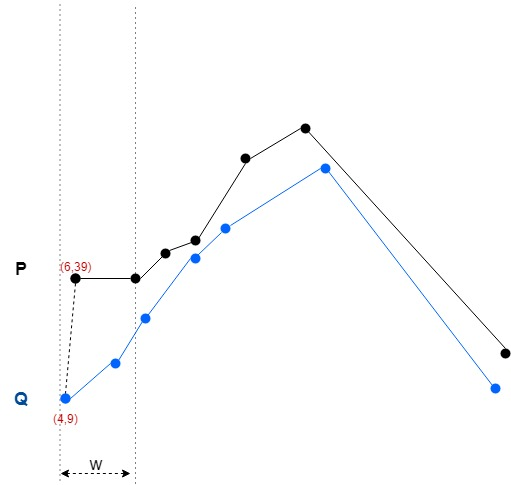
\includegraphics[width=0.45\textwidth]{Related_Works/related_trajes-wDF.jpg}
\caption{\label{fig:related_trajes_wDF}wDF score is the minimal distance of all maximal distances between two points within the given time window \textit{window}}
\end{figure}

In 2002, Vlachos \cite{vlachos2002discovering} proposed the \emph{Longest Common Subsequence} (LCSS) for raw trajectory similarity measuring, considering the spatial distance between two points. In LCSS, given a point $p$ of a trajectory $P$ and a point $q$ of a trajectory $Q$, they \textit{match} if the distance between them is less or equal to a given \textit{threshold} $\epsilon$, as can be seen in Equation \ref{func:match_LCSS}. LCSS reduces the effect of noisy data by quantifying the similarity between two points to binary values: 1 if the points match, and 0 otherwise. The longer the common subsequence of point matches between two trajectories, the more similar they are. 
A recursive formalization of LCSS is presented in Equation \ref{func:LCSS}{, that gives the total similarity of two trajectories $P$ and $Q$}.

\begin{equation}
%\scriptsize
\label{func:match_LCSS}
  match(p, q) = 
  \begin{cases} 
      true & dist(p_x, q_x)  \leq \epsilon\\ 
        &            \text{and } dist(p_y, q_y)  \leq \epsilon\\
      false & otherwise
  \end{cases}
\end{equation}

\begin{equation}
%\scriptsize
\label{func:LCSS}
  LCSS(P, Q) = 
  \begin{cases} 
      0 & \text{if } m = n = 0\\ 
      1 + LCSS(<p_2...p_m>,<q_2...q_n>) & \text{if } match(p_1, q_1)\\
      max(LCSS(<p_2...p_m>, Q),  & otherwise \\
      LCSS(P, <q_2...q_n>))
  \end{cases}
\end{equation}

A drawback of LCSS is its subsequence specificity, causing a inability to take into account gaps of any size in the trajectory. A  gap is a subsequence of points in a trajectory $P$ that is not close to any subsequence of points in a trajectory $Q$. Since the LCSS computation only takes into account the common/close points on both trajectories, this gap subsequence will not impact the computed similarity score. Figure \ref{fig:related_trajes_PQR} shows three trajectories $P$, $Q$, and $R$, with 3, 4, and 5 points, respectively. {As can be seen, the first point of trajectory $P$ matches with the first point of the trajectories $Q$ and $R$, since the distance between the points is less than the threshold $\epsilon$}. The total LCSS similarity of $P$ and $Q$ is $LCSS(P, Q) = 1$, while the similarity of $P$ and $R$ is also $LCSS(P, R) = 1$, even though two points of $R$ do not match any points of $P$.


\begin{figure}[h]
\centering
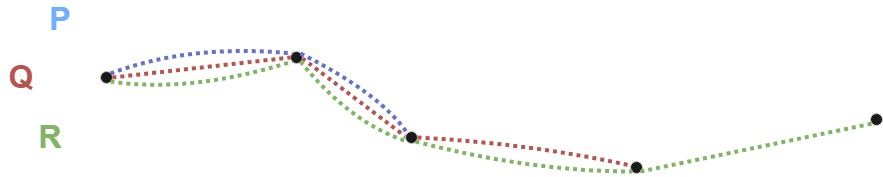
\includegraphics[width=0.9\textwidth]{Related_Works/related_trajes_PQR.jpg}
\caption{\label{fig:related_trajes_PQR}Trajectories $P$, $Q$ and $R$ have 3 points matching, while trajectories $Q$ and $R$ have 4 points matching.}
\end{figure}

The LCSS similarity score is given by the size of the longest common subsequence ($LCSS(P, Q)$) over the size of the shortest trajectory, i.e., $\dfrac{LCSS(P, Q)}{min(m, n)}$.
Figure \ref{fig:related_trajes_LCSS} shows the matching of points of trajectories $P$ and $Q$ considering a threshold $\epsilon =15$. The LCSS similarity score of $P$ and $Q$ is the number of points that match (solid black points) normalized by the size of the shortest trajectory, i.e. $\dfrac{4}{6} \approx 0.67 $.

\begin{figure}[h]
\centering
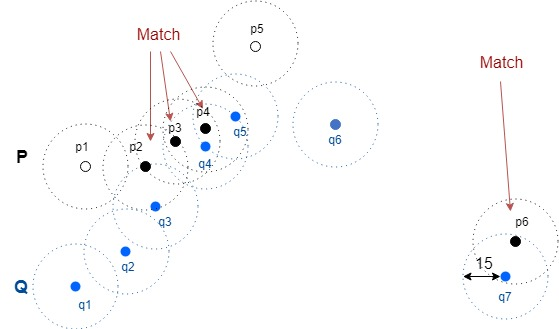
\includegraphics[width=0.45\textwidth]{Related_Works/related_trajes-LCSS.jpg}
\caption{\label{fig:related_trajes_LCSS}LCSS similarity score is the number of matched points normalized by the size of shortest trajectory.}
\end{figure}

Chen in \cite{Chen:2005:RFS:1066157.1066213} proposes the Edit Distance on Real sequence (EDR), another similarity measure for raw trajectories. EDR calculates the distance between two trajectories by computing the edit distance between their points. The edit distance between two trajectories is given by summing the distance between their points quantified as 1 if their points do not match, and 0 when they match (Equation \ref{func:match_EDR}). Using this approach, EDR solves the problem of the gaps in LCSS, by taking into account points that do not match. However, to enforce a match between two points EDR requires that their distance is below a given threshold in all dimensions.
A recursive  formalization of EDR is presented in Equation \ref{func:EDR}.

\begin{equation}
%\scriptsize
\label{func:match_EDR}
  match(p, q) = 
  \begin{cases} 
      0 & dist(p, q) \leq \epsilon \\ 
      1 & otherwise\\
  \end{cases}
\end{equation}

\begin{equation}
%\scriptsize
\label{func:EDR}
  EDR(P, Q) = 
  \begin{cases} 
      0 & \text{if } m = 0\\ 
      0 & \text{if } n = 0\\ 
      min(EDR(<p_2...p_m>,<q_2...q_n>) +  & otherwise\\
      match(p_1, q_1), EDR(<p_2...p_m>, Q) + 1, \\
      EDR(P, <q_2...q_n>) + 1) &
  \end{cases}
\end{equation}

The EDR similarity score is given by the inverse of the number of non-matched points over the size of the longest trajectory, i.e., $1 - \dfrac{EDR(P, Q)}{max(m, n)}$. In the example in Figure \ref{fig:related_trajes_EDR}, trajectories $P$ and $Q$ match in 4 of their points when using a threshold $\epsilon =15$. As an edit distance, EDR takes into account how many changes in one of the trajectories are necessary to transform one trajectory in the other. In this case, the trajectories have four common/close points. To make the trajectories look similar, the trajectory $P$ needs three changes in its points. For instance, 1) adding a new point similar to $q1$; 2) changing the point $p1$ to be close to the point $q2$; and 3) moving the point $p5$ closer to the point $q6$. The EDR similarity score of $P$ and $Q$ is the inverse of the total of non-matched points over the size of the longest trajectory, i.e. $1 - \dfrac{3}{7} \approx 0.57$.
This similarity score shows that EDR is robust to compare trajectories of different sizes, by giving distinct similarity scores for trajectories of different sizes, solving the drawback of LCSS. Moreover, EDR maintains the robustness to noise of LCSS by using a threshold value in all dimensions.

\begin{figure}[h]
\centering
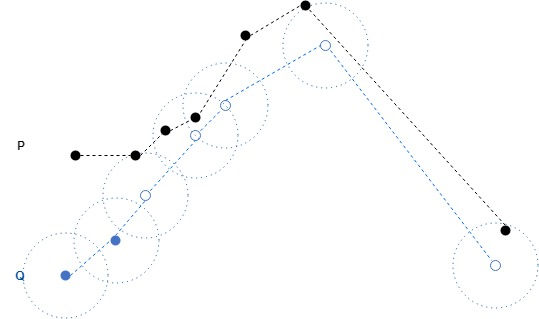
\includegraphics[width=0.45\textwidth]{Related_Works/related_trajes-EDR.jpg}
\caption{\label{fig:related_trajes_EDR}EDR distance score is the number of non-matched points normalized by the size of largest trajectory, subtracted by 1.}
\end{figure}

Very recently in 2018, Furtado proposed the \emph{Uncertain Movement Similarity} (UMS) in \cite{Furtado-UMS-2018}. UMS is a parameter-free similarity measure designed exclusively for raw trajectories, using only the spatial dimension. The main contribution of UMS is the elimination of parameters for similarity measuring, by defining a dynamic spatial threshold that is computed automatically according to the distance between the pairs of points of a trajectory. As a consequence, it solves the problem of irregular distribution of trajectory points. UMS represents trajectories as a sequence of movement ellipses, covering the space between two sampled trajectory points.
By using a dynamic ellipse size,  UMS avoids the definition of a radius of fixed size around each point, which is a problem for real applications where the sampling rate is normally irregular as the object changes its movement speed.

Figure \ref{fig:related_trajes_UMS} shows the trajectories $P$ and $Q$ represented as two elliptical trajectories according to UMS. UMS computes the similarity score taking into account three premises: i) \textit{alikeness}: {the number of $P$ ellipses that have some intersection with $Q$ ellipses plus the number of $Q$ ellipses that have some intersection with the $P$ ellipses}; ii) \textit{shareness}: the space covered by ellipses of trajectories $P$ and $Q$ have a big shared area; and iii) \textit{continuity}: the ellipses order represents moving objects traveling continually in the same direction. The limitation in this method lies in its inability to handle trajectories with higher sampling rate, because the higher the sampling rate of the points is, the smaller will be the generated ellipses, making the shared area between trajectories shorter.

\begin{figure}[!h]
\centering
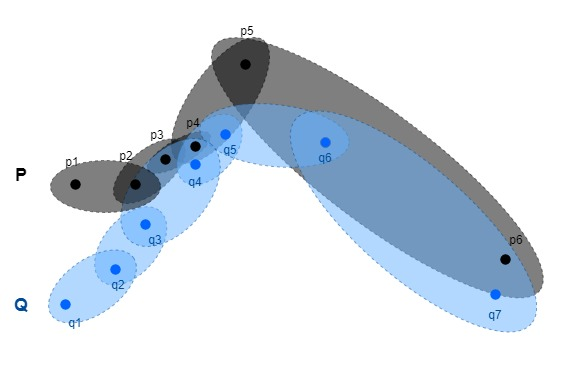
\includegraphics[width=0.75\textwidth]{Related_Works/related_trajes-UMS.jpg}
\caption{\label{fig:related_trajes_UMS}UMS similarity score is given by: i) the shape \textit{alikeness} of ellipses; ii) the \textit{shared} area of ellipses; and iii) the \textit{continuity} of points inside ellipses}
\end{figure}

\subsection{Related works on semantic trajectory similarity measures} \label{sec:related_semantic}

With the definition of semantic trajectory, the creation of new semantic-aware similarity measures become necessary. These new measures may analyze, besides the semantic information, any other information about the trajectory, as for instance the temporal duration of \emph{stops} and \emph{moves}, the moves spatial points, the average speed of the \emph{moves} and so on.
In the following we describe existing semantic trajectory similarity measures, as well as their limitations and applications. %In order to help understanding, we provide some examples, computing similarity scores using trajectories $P$ and $Q$, as previously illustrated in Figure \ref{fig:related_semantic_trajes}. These trajectories are annotated with the spatial coordinates of the \emph{stops} centroids, the time interval of each \emph{stop}, the name and type of the place where a \emph{stop} takes place, the name of the main street where the \emph{move} occurs, as well as the travelled distance and average speed during the \emph{move}.

An early similarity measure considering semantic trajectories is Common Visit Time Interval (CVTI) proposed in \cite{Kang:2009:SMT:1529282.1529580}. It was proposed as a measure for integrating the semantics {and the temporal dimensions of the stops}. It finds the Longest Common Subsequence of two semantic trajectories in which the semantics is the same and there is a time intersection between the stops. CVTI gives as similarity score the proportion of time that two trajectories share in the same \emph{stops}.
As CVTI is strongly based on LCSS, thus presenting the same drawback of LCSS: the inability to penalize gaps of any size in the trajectory. Although CVTI uses different data dimensions, the measure is not extensible for other data dimensions associated with \emph{stops} and \emph{moves}, since it handles exclusively the semantic and the time dimensions of \emph{stops}.

%Figure \ref{fig:related_trajes_CVTI} shows the comparison of two trajectories $P$ and $Q$ using the CVTI similarity measure. CVTI finds the Longest Common Subsequence (LCSS) of elements between both trajectories $P$ and $Q$ and gives as similarity score the proportion of time that both trajectories $P$ and $Q$ shared the same \emph{stops}.

%\begin{figure}[h]
%\centering
%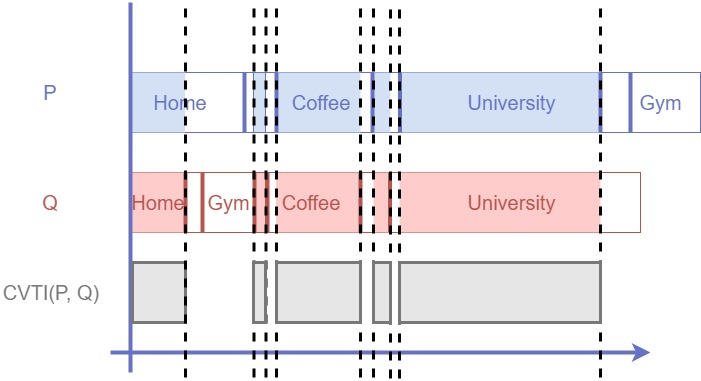
\includegraphics[width=0.65\textwidth]{Related_Works/Semantic_Trajectories_(CVTI).jpg}
%\caption{\label{fig:related_trajes_CVTI}CVTI similarity score is the longest common %subsequence with time intersection between two trajectories.}
%\end{figure}

In \cite{Ying:2010:MUS:1867699.1867703} the measure \emph{Maximal Semantic Trajectory Pattern Similarity} (MSTP) was proposed. It identifies the Longest Common Sequence (LCS) between two semantic trajectories, which are sequences of labels describing the types of places such as $<School, Park, Cinema>$. {MSTP uses only the semantic dimension of the trajectories, not being extensible for multiple dimensions, as time and space.} MSTP differentiates from LCSS because it computes a ratio between each trajectory and their common patterns, i.e. the sequence of places visited by both trajectories. The average ratio is used to compute the similarity score, avoiding the drawback of LCSS that does not differentiate matching gaps of different sizes. {The main limitation of the method lies in the exclusively semantic focus, being not extensible to multiple dimensions.}

The work of \cite{Liu:2012:SMM:2442968.2442971} proposed a semantic similarity measure that combines two distances: geographic and semantic. The geographic distance considers three aspects: (i) the distance between the centroids of the trajectories; (ii) the difference in the length of the trajectories; and (iii) the cosine similarity of the directions of subtrajectories. The measure uses the speed variation between the \emph{stops} to split trajectories into subtrajectories. The semantic distance is based on LCSS to find the longest common subsequence of \emph{stops} that were visited by the individual. Limitations of this approach include: i) sensibility to noise in the geographic distance; ii) the time distance is not considered; and iii) the prevalence of the geographic distance, i.e. two trajectories are similar only if they are similar in space.

The \emph{Maximal Travel Match} (MTM)\cite{Xiao:2010:FSU:1869790.1869857} analyzes the trajectory similarity in the semantic dimension constrained by time. In order to do that, MTM takes into account the semantics of the visited places (e.g., restaurant, university etc.), the sequence of the these places, the traveled time between places, and the frequency that a place was visited. Two trajectories are more similar if they visited places of the same type, in the same order, with similar travel times, according to a time threshold. Limitations of this approach include: i) two semantic trajectories are similar only if they visit the places in the same order; ii) the space dimension is not considered; and iii) MTM measures the similarity considering the whole dataset in order to obtain the frequency of the visited places, what makes the result dependent of the other trajectories in the dataset.

In the work of \cite{Furtado:TGIS12156}, the MSM (Multidimensional Similarity Measure) was proposed. This measure is the first in the literature working with multiple dimensions. MSM was designed to handle multidimensional sequences, in which each dimension is independent and each dimension should have its own distance function. 
MSM uses a threshold value for defining if two elements match in a dimension or not\hl{, as can be seen in Equation {\ref{func:match_MSM}}.}

\begin{equation}
\label{func:match_MSM}
  match_d(a, b) = 
  \begin{cases} 
      1 & dist_d(a, b) \leq maxDist_d \\
      0 & otherwise
  \end{cases}
\end{equation}

\hl{Equation {\ref{func:MSM_score}} presents how MSM computes the similarity score between all possible pairs of \emph{stops} of two trajectories. For each pair of \emph{stops}, MSM sums the matching value for all \emph{D} dimensions and multiplies it by a pre-defined importance weight $w_d$ for each dimension. With this, MSM supports to assign more or less relevance for each dimension, based on the application needs.}

\begin{equation}
\label{func:MSM_score}
score(a, b) = \sum\limits_{d=1}^D match_d(a, b) * w_d
\end{equation}

\hl{To compute the similarity score between two trajectories, initially MSM calculates the \emph{parity} between them, as Equation {\ref{func:MSM_parity}} shows. The parity score is given by summing the highest similarity scores of all stops $a$ of the trajectory $A$ when compared with all stops $b$ of the trajectory B.}

\begin{equation}
\label{func:MSM_parity}
parity(A, B) = \sum\limits_{a\in A} \textbf{max}\{\textit{score}(a, b) : b \in B\}
\end{equation}

\hl{As the parity value is the number of commonalities between two trajectories \emph{A} and \emph{B}, MSM computes the final similarity score between them as the average of their parity values by the number of \emph{stops} in both trajectories, as presented in Equation {\ref{func:MSM}}.}

\begin{equation}
\label{func:MSM}
\begin{split}
  MSM(A, B) = 
  \begin{cases} 
      0 & if  |A| = 0 \vee |B| = 0 \\
      \frac{parity(A, B) + parity(B, A)}{|A| + |B|} & otherwise
  \end{cases}
\end{split}
\end{equation}

\hl{With this approach, MSM can take into account distinct dimensions, such as space, time, and semantics, to be scored in an one similarity value and it supports to define individual importance weights for each dimension.}
Some limitations of this approach include: i) the elements homogeneity allows MSM to handle \textit{stops} only, since \textit{stops} and \textit{moves} have distinct attributes, and ii) the order of the elements is not taken into account during the similarity calculation.

Figure \ref{fig:related_trajes_MSM} shows the comparison of two semantic trajectories $P$ and $Q$. In this figure, MSM scores the similarity in a pair-wise fashion, comparing all \emph{stops} of trajectory $P$ with all \emph{stops} of trajectory $Q$. Its compares each dimension of the stops (space, time, and semantics), using a specific distance function for each dimension. After all stop-to-stop comparisons, MSM computes the similarity score as the sum of the best matching score of each \emph{stop}, both $P$ and $Q$ trajectories, over the sum of trajectories length. \hl{In this example, MSM highly scores the similarity of the two trajectories, since both trajectories basically visit the same places, both  spatially and semantically, and stay on the \emph{stops} at approximately the same time. Notice that the sequence of the visited \emph{stops} is very different between the two trajectories, but MSM does not take this into account.}

\begin{figure}[h]
\centering
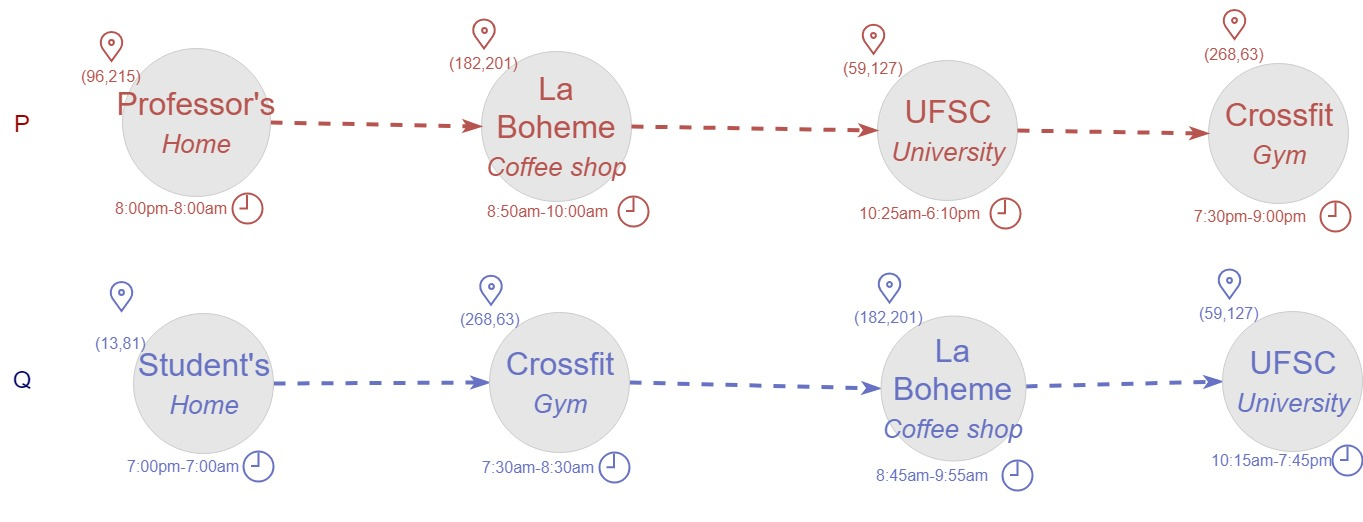
\includegraphics[width=0.9\textwidth]{Related_Works/Semantic_Trajectories_(MSM).jpg}
\caption{\label{fig:related_trajes_MSM}MSM similarity measure computes the similarity score of $P$ and $Q$ using multiple dimensions with partial matching.}
\end{figure}

Cai in \cite{CaiLee2016} proposed a measure that combines the strategies of LCSS \cite{vlachos2002discovering} and MSM\cite{Furtado:TGIS12156} for semantic trajectories. It finds the longest common subsequence between two semantic trajectories. The difference to LCSS is that it does not require the matching in all dimensions, and it does separate the dimensions in two types: required or optional. While all required dimensions should be similar for two points to match, the optional ones are used only to increase the score. \hl{It uses weights for the optional dimensions, so if two points match in one relevant dimension, but does not match in other dimensions, their similarity are greater than when compared with another point that matches in a less relevant dimension.}

Table \ref{tab:comparative_table} summarizes the main characteristics of most related measures in comparison to the measure proposed in this thesis. We group the measures in two distinct categories: raw or semantic trajectory similarity.

We compare all measures considering: i) if the similarity comparison is performed comparing all possible pairs of points by the measure (pair-wise); ii) the computational complexity; iii) if the computation of the distance between points is match-based or is continuous (i.e., Euclidean distance, Hausdorff distance, etc); iv) if the measure is robust to noisy data; and v) if the measure is extensible to support multiple dimensions (space, time, and semantics); and vi) if the measure takes into account the sequence of the points in total, partially, or without order.

When comparing the similarity measures for semantic trajectories, we consider: i) if the measure takes into account the \emph{stops} of the trajectory; ii) if the measure takes into account the \emph{moves} of the trajectory; iii) if the measure allows the use of weights for the dimensions; and iv) if the measures gives a partial score when elements of two trajectories do not match in all dimensions.

\begin{landscape}
    \begingroup
        \setlength{\tabcolsep}{6pt} % Default value: 6pt
        \renewcommand{\arraystretch}{1.5} % Default value: 1
        \vspace*{\fill}
        \begin{table}[h!]
        \scriptsize
          \centering
          \begin{tabular}{|l|c|c|c|c|c|c|c|c|c|c|c|c|c|}
          	\hline
          	    & \multicolumn{5}{c|}{Raw trajectory similarities} & \multicolumn{7}{c|}{Semantic trajectory similarities}\\
          	\hline
        		& DTWa & wDF & LCSS & EDR & UMS & CVTI & MSTP & Liu & MTM & MSM & Cai & SMSM\\
          	\hline
             Pair-wise similarity & \checkmark & \checkmark & \checkmark & \checkmark & \checkmark & \checkmark &  & \checkmark &  & \checkmark & \checkmark & \checkmark \\
          	\hline
             Computational-complexity & $n^2$ & $n^2$ & $n^2$ & $n^2$ & $n^2$ & $n^2$ & $n^2$ & $n^2$ & $n^2$ & $n^2$ & $n^2$ & $n^2$\\
          	\hline
             Matching threshold &  &  & \checkmark & \checkmark &  &  &  & \checkmark&  & \checkmark& \checkmark& \checkmark\\
          	\hline
             Robust to noise &  &  & \checkmark & \checkmark &  & \checkmark & \checkmark & \checkmark & \checkmark & \checkmark & \checkmark & \checkmark \\
          	\hline
             Space dimension & \checkmark & \checkmark & \checkmark & \checkmark & \checkmark &  & \checkmark & \checkmark & \checkmark & \checkmark & \checkmark & \checkmark\\
          	\hline
             Time dimension & & \checkmark & \checkmark & \checkmark &  & \checkmark & \checkmark &  & \checkmark & \checkmark & \checkmark & \checkmark\\
          	\hline
             Semantic dimension &  &  &  &  &  & \checkmark & \checkmark & \checkmark & \checkmark & \checkmark & \checkmark & \checkmark\\
          	\hline
             Full sequence & \checkmark & \checkmark &  &  &  &  &  &  &  &  &  & \\
          	\hline
             Partial sequence &  &  & \checkmark & \checkmark & \checkmark & \checkmark & \checkmark & \checkmark & \checkmark &  &  & \checkmark\\
          	\hline
             No sequence &  &  &  &  &  &  &  &  &  & \checkmark & \checkmark & \\
          	\hline
             Support stops &  &  &  &  &  & \checkmark & \checkmark & \checkmark & \checkmark & \checkmark & \checkmark &\checkmark \\
          	\hline
             Support moves &  &  &  &  &  &  &  &  &  &  &  & \checkmark \\
          	\hline
             Dimension weighting &  &  &  &  &  &  &  &  &  & \checkmark & \checkmark & \checkmark \\
          	\hline
             Partial matching &  &  &  &  &  &  &  &  &  & \checkmark & \checkmark & \checkmark\\
          	\hline
          \end{tabular}
          \caption{Comparative table}
          \label{tab:comparative_table}
        \end{table}
        \vspace*{\fill}
    \endgroup
\end{landscape}
